Developing an effective solution for \glspl{VDM} requires addressing key challenges related to dataset availability, document structure variability, and generalization to unseen layouts. This section provides a detailed description of these components and the experimental procedures used to evaluate their effectiveness. Figure~\ref{fig1} illustrates the proposed methodology, outlining the sequential steps from dataset preparation to result analysis.

% This study follows an applied research approach, aiming to tackle practical challenges in \glspl{VDM} for document understanding tasks. The research is primarily quantitative, as it assesses model performance using objective metrics. We conduct experiments to evaluate our \glspl{VDM} method and compare its performance against alternative approaches. Additionally, the problem of generalizing structural document patterns in zero-shot settings remains underexplored in the literature, further motivating this investigation.

% The study adopts a computational modeling approach, involving the development of an algorithm for zero-shot \gls{DLR}. The methodology encompasses dataset construction, learning architecture design, and experimental validation through structured evaluation protocols. Figure~\ref{fig1} illustrates the proposed methodology, outlining the sequential steps from dataset preparation to result analysis.

\begin{figure}[htbp]
\centering
%\isPreprints{\centering}{} % Only used for preprints
\includegraphics[width=\textwidth, trim={0em 0em 0em 0em},clip]{images/Pipeline Pesquisa 1.png}
\caption{Overview of the proposed \glsfirst{LA-ZSL} methodology for \glsfirst{VDM}.\label{fig1}}
\end{figure}  

\section{Dataset Construction}
\label{sec:method_dataset}

The OL-CDIP proposed dataset is built as a reorganization of the RVL-CDIP \cite{harley2015rvlcdip} dataset. While RVL-CDIP's classes are divided by their meaning and written content of the documents, our dataset is divided by the visual information and layout. This is illustrated in Figure \ref{img:dataset}, where both groups of documents are classified as the same class under RVL-CDIP, both being forms, but are re-arranged to be different classes under OL-CDIP, as they are visually distinct. 

\begin{figure}[htbp]
%\isPreprints{\centering}{} % Only used for preprints
  \centering
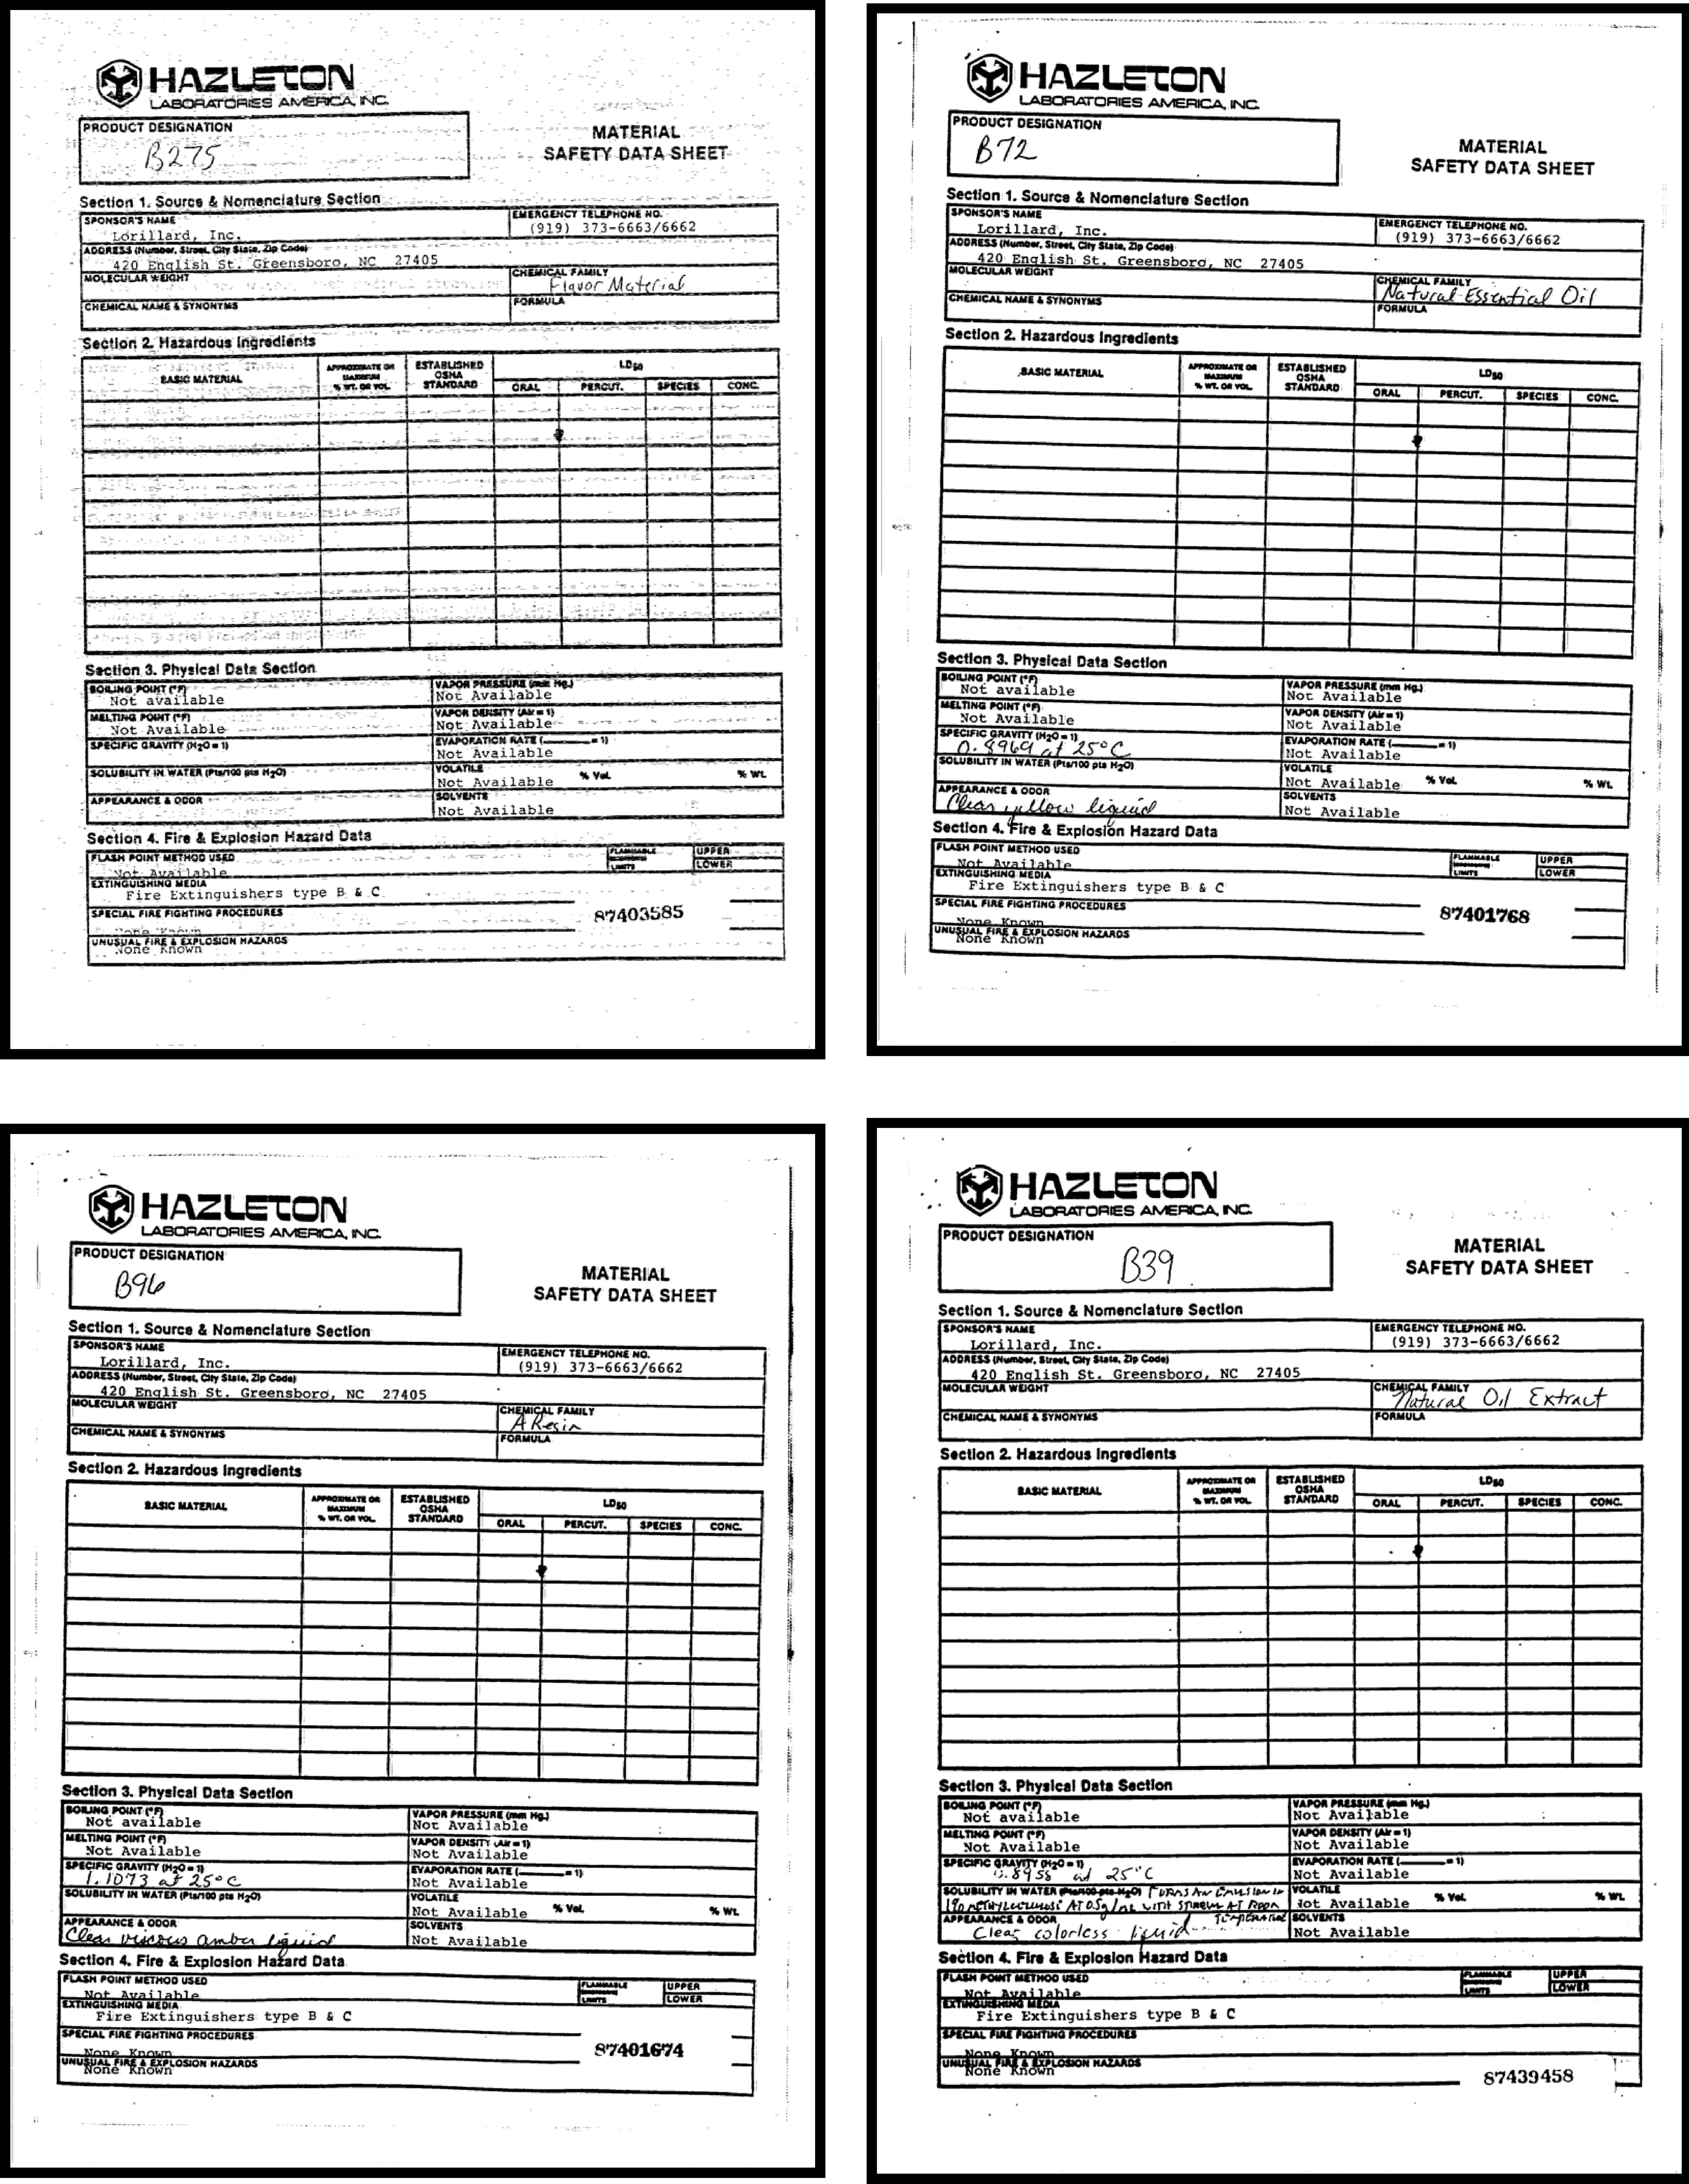
\includegraphics[width=.4\textwidth]{images/class_comparison1.png} \hspace{.1\textwidth}
        % [.1\textwidth] % espaço vertical entre as imagens
    \includegraphics[width=.4\textwidth]{images/class_comparison2.png}

\caption{Examples of two distinct classes under the proposed \gls{LA-CDIP} dataset. Those classes originally belonged to the same class under RVL-CDIP organization.\label{img:dataset}}
\end{figure}   

The construction of the database followed 2 stages: preliminary clustering, followed by a manual reorganization. The clustering is made with a private metric learning model, trained with a private document dataset, using a similar framework as the one presented here. The clustering is made possible by the metric learning nature of the solution, as the output of the trained model is a feature value in a feature space. The clustering algorithm used was Hierarchical Agglomerative Clustering, with Ward\cite{ward1963} strategy. The clustering served exclusively as suggestions, as the cluster themselves were not homogeneous, neither were unique. Then, we manually reorganized and labeled the clusters, grouping primarily by the visual layout information. Next, we conducted a second independent validation of the dataset, reviewing both intra-class and inter-class consistency.

To maintain train-test data consistency, we split the data e follow the \gls{ZSL} and \gls{GZSL} protocols proposed by Xian et al \cite{gzsl}. Each protocol is a different method to split train and test data: \gls{ZSL} is the complete separation of train and test classes - no overlap between the splits; while the \gls{GZSL} follows a more realistic scenario by partially overlapping train and test classes, having half the test or validation set be of seen classes, and half of unseen classes. In both scenarios, we split the data into train and test data, and the train data is further divided by a 5-fold cross-validation \cite{kfoldcv}.

The data for the test scenario and the data for each split are chosen randomly, and the same for every experiment. The test scenario is picked as a sixth split for the cross-validation, so it follows the same rules for the other 5 splits. For the \gls{ZSL} scenario, a sixth of the classes are randomly chosen for each split, with no overlapping. Naturally, this scenario creates splits with variable sizes, as the classes themselves have variable sizes. For the \gls{GZSL} scenario, half the classes in the whole dataset are chosen as classes that do not overlap between splits, and other half are diluted between the splits. While constructing a split, first, we choose the non overlapping classes for the split, then we fill the remaining slots with the overlapped classes, achieving splits with a constant size for this scenario.

This dataset can be used for a traditional visual classification problem, but since we tackle it with metric learning, additional considerations must be taken into account. While using a Siamese network, running inference on a single point of data returns no information, as the architecture requires some sort of comparison between different data points. Randomly selecting pairs every test can fluctuate the results, therefore, to maintain the test consistency, we wrote a test protocol that assures the same pairs are tested every time. For every document in the set, we chose two other documents: one that shares the same class, and one that does not. This document is chosen randomly by its class, therefore, every class has the same probability of being picked. A protocol exists for the test set and for every cross-validation split.

\section{Leveraging LLM for Benchmarking Visual Document Matching}
\label{sec:method_benchmark}

\glspl{LLM} have demonstrated their ability to perform zero-shot classification in various domains, including document understanding. Scius-Bertrand et al.~\cite{scius2024zeroshot} show that GPT-4 with vision capabilities can classify documents from the RVL-CDIP data set with almost 70\% accuracy without requiring task-specific fine-tuning or reliance on \glspl{OCR}.

With the need to process multimodal information, there has been a rapid advancement in models with visual capabilities. Llama 3.2 Vision ~\cite{meta2024llama3.2}, for example, was introduced as an open source alternative with multimodal reasoning capabilities. Other recent work has analyzed the relationship between performance and efficiency. In 2024, DeepSeek-VL2~\cite{DBLP:journals/corr/abs-2412-10302} exemplified this trend, achieving competitive results with fewer activated parameters compared to models such as InternVL2 and Qwen2-VL.

In 2025, InternVL 2.5 was introduced as an evolution of its predecessor, InternVL 2.0, incorporating enhancements that resulted in performance gains, and InternVL 2.5 exceeded 70\% accuracy on the MMMU benchmark, setting a new standard for open source multimodal models~\cite{internvl2024}. Moreover, its performance is competitive with leading proprietary models, such as OpenAI’s GPT-4o\cite{openai2024gpt4o,openai2024gpt4omini}.
In 2025, Qwen2.5-VL was introduced as an evolution of the Qwen2-VL series, surpassing its predecessor. According to its evaluation~\cite{bai2025qwen2}, Qwen2.5-VL excels in OCR-related tasks, chart interpretation, and document understanding. The leadership in state-of-the-art performance for these benchmarks is now primarily held by GPT-4o, InternVL 2.5, and Qwen2.5-VL, the latter two representing the strongest open-source alternatives.

Given their ability to understand zero-shot documents, we evaluate the multimodal \glspl{LLM} Llama 3.2 Vision, InternVL 2.5, Qwen2.5-VL, GPT-4o-2024-11-20 and GPT-4o-mini-2024-07-18. We also tested DeepseekVL2, which, like the others, supports multiple images; however, in its small version, it did not demonstrate the ability to distinguish between similar and different document pairs and was therefore not included in the comparison.

To benchmark \glspl{VDM}, we design a structured prompt that guides \gls{LLM} to compare two document images, evaluating visual similarity. Models were asked to assign a similarity score from 0 to 100, categorized into five levels: Nearly Identical, Highly Similar, Moderately Similar, Weak Similarity, and Completely Different. This evaluation was carried out using Google Colab~\cite{googlecolab}, where the size of the model and the computational resources were limited. \refFig{fig:document_comparison} illustrates the input-output structure of our document comparison framework. The left and right images represent the document pairs analyzed by \glspl{LLM}, which generate a similarity score and a categorical classification.

\begin{figure}[htbp]
    \centering
    \includegraphics[width=.8\linewidth]{images/similar.png}
    % \caption{Comparison of two similar documents}
    % \label{fig:document_comparison1}
    \\[1em]
% \end{figure}
% \begin{figure}[htbp]
    \centering
    \includegraphics[width=.8\linewidth]{images/different.png}
    \caption{Two sets of comparisons by a LLM model. In the first example, we show the same layout, and in the second, different layouts. The scores range from 0 to 100.}
    \label{fig:document_comparison}
\end{figure}

To ensure a fair evaluation, both models are tested on 1,036 protocol documents from one dataset and 1,652 from another, assessing their \gls{VDM} ability. This comparison aims to determine the feasibility of using \glspl{LLM} for \gls{ZSL} \gls{VDM} and serves as a baseline for evaluating the performance and efficiency of our proposed method.

\section{Modeling}
\label{sec:method_modeling}

%cluster
%pair
Traditional classification methods, such as entropy learning, locks the generality of the model to the set of classes it has been trained on. Therefore, we use Zero Shot Learning techniques to be able to classify document layouts that have not been seen on the training set. To experiment on our dataset, we use a wide variety of Backbones for our trainings, but they all follow the same metric learning architecture with Siamese Networks.

% \blue{We use well established computer vision architectures on our experiments as backbones} \red{<- isso aqui precisa ser melhor explicado: como você faz isso? O que seu método se diferencia do mero uso dessas arquiteturas como classificadores? Use equações e diagramas para ilustrar isso. Está faltando muita informação para um leitor entender o que são esses backbones e o que é o seu método.} for the Siamese network.
We benchmark our dataset choosing traditional, well established vision Neural Networks as our Backbones. They are ResNet~\cite{he_deep_2016}, MobileNetV3~\cite{howard_searching_2019}, EfficientNet~\cite{tan_efficientnet_2019}, VGG~\cite{simonyan_very_2015}, \gls{ViT}~\cite{dosovitskiy_image_2021}. To adapt the architectures to a siamese network, we change only the last linear layer of each model---the classification layer---into a new linear layer with an arbitrary size $n$, suitable for our problem. Intuitively, the model learns to draw a representation of a input document in a feature space with $n$ dimensions, such that documents that share the same class are represented clustered together, and documents that have different classes are far apart. 

Our trained models are exclusively visual, therefore, their input data is the $(R, G, B)$ document image matrix. First, we resize the input image to a shape compatible with each neural architecture. For most models, this is a $(224, 224)$ height and width. EfficientNet is the only architecture that does not follow this rule, as the different model versions increase their input size at the same time they increase the network depth and width. Then, every value of the image matrix is scaled from $0-255$ to $0-1$, and normalized with the mean and standard deviation of the current training split. During a training epoch, for each document in the dataset, a random document is chosen to close a pair. Every class has the same odds of being chosen to mitigate overfit in predominant classes. We use no data augmentation and no pair mining.

We train these models with a supervised contrastive learning framework, and use the Contrastive Loss~\cite{chopra_learning_2005} as our loss function. It's objective is to minimize the distance between two elements of the same class, but increase the distance otherwise. Given a sample pair $\{(a, b)\}$ of feature spaces, and $y$ as a label with value $1$ if $a$ and $b$ share the same class, $0$ otherwise, we have
\begin{equation}
        Loss = y * d(a, b)^2 + (1 + (-1 * y)) * abs(m - d(a, b))^2,
\end{equation}
where $d$ represents a metric function and $m$ a hyperparameter defining the lower bound distance between samples of different classes. In this context of this paper, $m$=$0.5$ and $d$ is the Euclidean distance between two points $P = (x_1, x_2, \cdots, x_n)$ and $Q = (y_1, y_2, \cdots, y_n)$ in an $n$-dimensional space defined mathematically as:
\begin{equation}
d(P,Q)={\sqrt {(x_{1}-y_{1})^{2}+ \cdots +(x_{n}-y_{n})^{2}}} = \sqrt{ \sum_{i=1}^{n} (x_i - y_i)^2 }.
\end{equation}